\section{Методика расчёта}

\subsection{Расчётная ячейка границы}

Все расчёты выполнены в пакете LAMMPS (версия 22.07.2025, сборка
KOKKOS\slash CUDA для графических процессоров) [8]. Межатомные силы заданы
потенциалом 2NN-MEAM (модифицированный метод погружённого атома с учётом
вторых соседей) Елинека и др. для системы Al--Si--Mg--Cu--Fe [9] --- единым
потенциалом, который описывает все атомы ячейки, в том числе атомы по обе
стороны границы, одним набором правил взаимодействия.

Матрица --- ГЦК (гранецентрированный кубический) алюминий
($a = 4{,}05$~\AA{}). Её ориентация, $x\parallel[1\bar{1}0]$,
$y\parallel[11\bar{2}]$, $z\parallel[111]$, продиктована системой скольжения
ГЦК-алюминия: дислокации в алюминии движутся по плоскостям $\{111\}$ вдоль
направлений $\langle110\rangle$, и при таком выборе плоскость скольжения
(111) параллельна границе, а направление скольжения $[1\bar{1}0]$ лежит
вдоль $x$. Краевая дислокация (край лишней атомной полуплоскости, вставленной
в кристалл) с вектором Бюргерса $\tfrac{1}{2}[1\bar{1}0]$ --- трансляцией
решётки, задающей переносимое ею смещение, $|\mathbf{b}| = 2{,}86$~\AA{}, ---
и линией вдоль $y$ при этом проходит через всю ширину ячейки, представляя
бесконечно длинную прямолинейную дислокацию, и скользит вдоль $x$
параллельно границе; именно такое движение и должен вызывать проверяемый
механизм.

Включение --- моноклинный интерметаллид Al$_{13}$Fe$_4$ со структурой из
работы [10]. Оно построено как плоский слой толщиной 20~\AA{}, несущий на
верхней поверхности полуэллиптический выступ (далее --- гребень) с полуосями
35~\AA{} вдоль $x$ и 20~\AA{} вдоль $z$, протянутый через всю ячейку вдоль
$y$. Гребень необходим: плоский деформированный слой, занимающий всю ячейку,
снимает нормальное напряжение простым расширением вверх, и именно
искривлённые края гребня создают в матрице неоднородное поле напряжений ---
так же, как его создавала бы кривизна поверхности реальной частицы. Плоский слой оставлен недеформированным, деформацию несёт только гребень
(раздел~2.2).

Вдоль $x$ и $y$ ячейка периодична: атом, выходящий через одну грань, входит
через противоположную, так что ячейка представляет неограниченную в плоскости
границу. Размеры в плоскости ($L_x = 154{,}64$~\AA{}, $L_y = 64{,}48$~\AA{}: 54 и
13 периодов решётки алюминия, десять и восемь ячеек Al$_{13}$Fe$_4$) выбраны
так, чтобы обе решётки были периодичны в плоскости. Малое остаточное
несоответствие ($-0{,}22\%$ вдоль $x$, $-0{,}26\%$ вдоль $y$) отнесено к
включению и одинаково в деформированной и контрольной ячейках, поэтому при их
сравнении оно сокращается в первом приближении. Атомы алюминия, оказавшиеся ближе
2{,}2~\AA{} к атому включения (с учётом периодических образов), удалены;
наименьшее межатомное расстояние в полученной структуре составляет
2{,}22~\AA{}. Толщина слоя алюминия над плоскостью границы 129~\AA{} (56 атомных
плоскостей (111)), ячейка в целом содержит 91\,428 атомов (72\,532 в матрице
и 18\,896 во включении); вдоль $z$ она ограничена сверху свободной
поверхностью и 17~\AA{} вакуума, снизу --- слоем толщиной 6~\AA{}, атомы
которого закреплены (рис.~\ref{fig:cell}).

Включение сцеплено с матрицей. Атомы по обе стороны границы взаимодействуют
через один и тот же потенциал, никаких ограничений или искусственной связи на
границе не вводится, и граница не проскальзывает и не раскрывается иначе, чем
через смещения атомов, допускаемые самим потенциалом. Контрольная структура релаксируется в три стадии: минимизация энергии
методом сопряжённых градиентов (атомы переводятся в положения минимума
энергии без теплового движения), 6~пс молекулярной динамики при 300~К с
последующим охлаждением до 0{,}5~К за 12~пс, снимающие длинноволновые моды
слоя, недоступные одной минимизации, и заключительная минимизация до силы
0{,}05~эВ/\AA{} (2-норма по всем атомам). Деформированная ячейка строится из
этого релаксированного состояния (раздел~2.2) и минимизируется до
0{,}02~эВ/\AA{}.

\begin{figure}[!htbp]
\centering
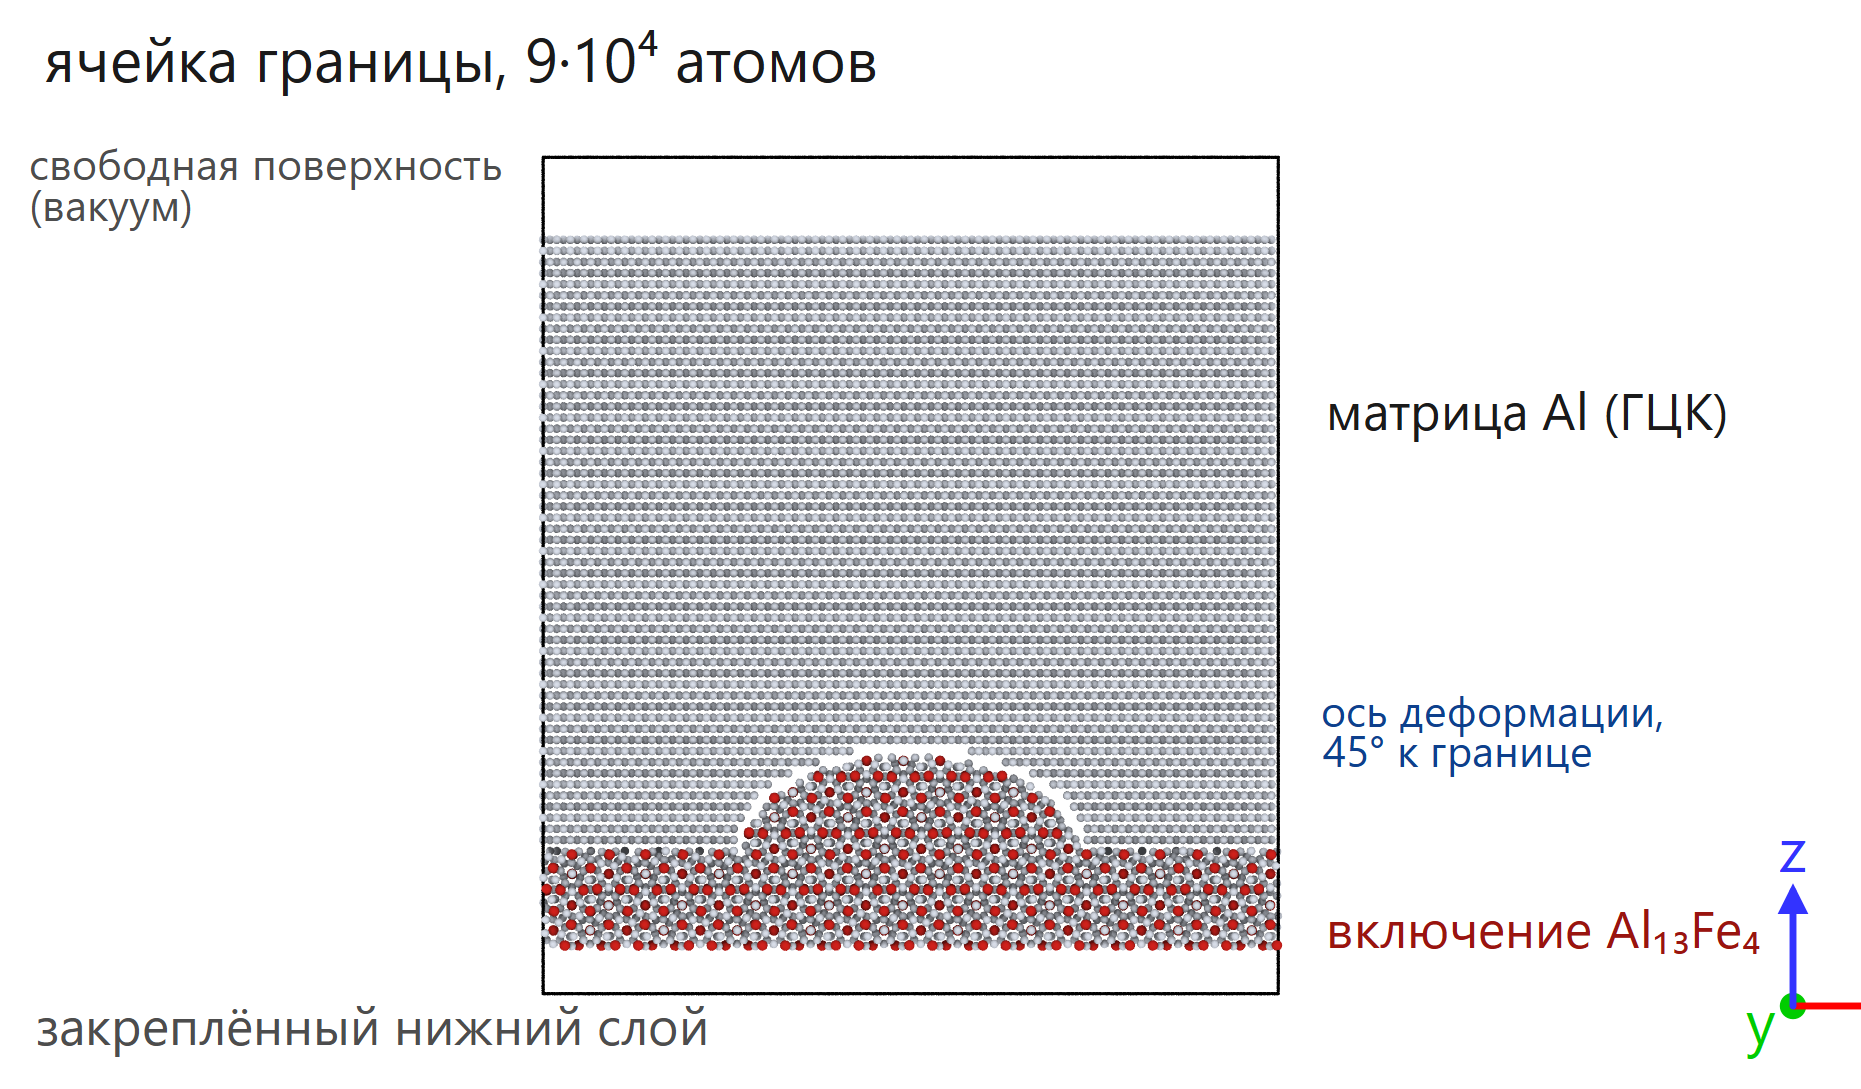
\includegraphics[width=0.92\linewidth]{fig_cell_interface_ru}
\caption{Расчётная ячейка границы в проекции вдоль $y$ (плоскость
$x$--$z$). Серым показана матрица алюминия --- 129~\AA{} ГЦК-алюминия с
осями $x = [1\bar{1}0]$, $y = [11\bar{2}]$, $z = [111]$, так что граница
параллельна плоскости скольжения (111), а $x$ --- направление скольжения.
Красным --- включение Al$_{13}$Fe$_4$: плоский слой с полуэллиптическим
гребнем шириной 70~\AA{} и высотой 20~\AA{}. Нижние 6~\AA{} включения
закреплены; над алюминием --- вакуум. Ячейка периодична вдоль $x$ и $y$.
Наложенное удлинение включения направлено под $45^{\circ}$ к границе в
плоскости $x$--$z$.}
\label{fig:cell}
\end{figure}

\subsection{Представление действия поля}

Молекулярная динамика --- классическая механика, и само магнитное поле в
расчёте отсутствует. Его действие представлено механически --- деформацией,
которую оно, по предположению, вызывает во включении. Вслед за
предшествующими экспериментальными работами [3--6], в которых поле действует
через магнитострикцию, то есть удлинение включения вдоль направления поля,
включение принято удлиняющимся вдоль направления поля $\mathbf{u}$ на
$\varepsilon = 1{,}94\cdot10^{-3}$ (0{,}194\%) --- упругую деформацию
$\sigma_m/E_{\mathrm{Al}}$ (при $E_{\mathrm{Al}} = 75{,}7$~ГПа), отвечающую оценённому в этих работах напряжению
на границе $\sigma_m = 147$~МПа [5], --- при постоянном объёме: удлинение
$\varepsilon$ вдоль $\mathbf{u}$ и сжатие на $\varepsilon/2$ вдоль двух
перпендикулярных направлений. В тензорной записи
\begin{equation}
\varepsilon^{*}_{ij}
  = \tfrac{3}{2}\,\varepsilon\!\left(u_i u_j - \tfrac{1}{3}\delta_{ij}\right),
\qquad \operatorname{tr}\varepsilon^{*} = 0,
\end{equation}
где $\delta_{ij}$ равно 1 при $i = j$ и 0 в остальных случаях, а нулевой след
выражает постоянство объёма. В теории упругости включений деформацию такого
рода --- ту, которую включение приняло бы, будучи свободным от матрицы, ---
называют собственной деформацией [7]; ниже этот термин употребляется именно в
этом смысле. Принятое значение существенно превышает магнитострикцию,
измеренную в сплавах Fe--Al [11,\,12]; оно используется потому, что это та
амплитуда, которую предполагает сам предложенный механизм, и механизм
проверяется при ней.

Направление $\mathbf{u}$ наклонено под углом $45^{\circ}$ к нормали границы
в плоскости $x$--$z$. Причина геометрическая. При $\mathbf{u}$ вдоль нормали
$z$ наложенная деформация не создаёт на системе скольжения $(111)[1\bar{1}0]$
никакого касательного напряжения: фактор Шмида (геометрический множитель,
переводящий напряжение в касательное напряжение на данной системе скольжения)
равен нулю точно, и на дислокацию, скользящую параллельно границе, не
действовала бы никакая сила. При $45^{\circ}$ сдвиговая составляющая
наложенной деформации на плоскости скольжения максимальна,
$\varepsilon^{*}_{xz} = \tfrac{3}{4}\varepsilon = 1{,}46\cdot10^{-3}$. В
поликристалле на поле откликаются те зёрна, чьи плоскости скольжения
благоприятно наклонены к нему, и наклонённая ячейка представляет именно эту
часть зёрен. Наклон одинаков во всех ячейках.

Деформация задаётся смещением каждого атома гребня относительно центра
гребня пропорционально его положению,
$\mathbf{r} \rightarrow \mathbf{r} + \varepsilon^{*}\!\cdot\!\mathbf{r}$, что
однородно растягивает гребень вдоль $\mathbf{u}$ и сжимает поперёк
$\mathbf{u}$. Плоский слой под гребнем оставлен недеформированным. Он
проходит через всю периодическую ячейку, а слой, периодичный в своей
плоскости, нельзя когерентно сдвинуть: удерживаемый при сдвиге формулы~(1),
он имел бы поверхность в виде пилы со ступенькой
$\varepsilon^{*}_{xz}L_x = 0{,}22$~\AA{} на границе ячейки, и весь слой
алюминия над ним оказался бы растянут вдоль $z$ примерно на
$\varepsilon^{*}_{xz}$ --- напряжение порядка 150~МПа по всей ячейке, что и
наблюдалось при такой попытке. Гребень --- та частица, поле которой
измеряется; слой лишь замыкает ячейку. Межатомный потенциал не изменяется. Поле напряжений,
создаваемое деформированным включением, получается как разность между ячейкой
с деформированным включением и контрольной ячейкой без деформации,
минимизированными из одинаковых исходных структур в одинаковых условиях.
Рассчитаны два варианта, различающиеся тем, позволено ли включению
релаксировать.

В варианте \emph{с удерживаемой деформацией} каждый атом включения ---
гребень в смещённом положении, плоский слой в исходном --- удерживается
жёсткой пружиной (жёсткость 20~эВ/\AA$^{2}$, что удерживает атом в пределах
примерно 0{,}01~\AA{} от этого положения), пока матрица релаксирует вокруг
него, так что гребень сохраняет деформацию~(1) на всём протяжении расчёта. В
соответствующей контрольной ячейке пружины подключены точно так же, поэтому
в разности двух ячеек они сокращаются. Эта ячейка даёт поле напряжений
частицы, поддерживающей свою собственную деформацию. Под действием сил, возникающих на границе, атомы включения отходят от
заданных положений примерно на 0{,}01~\AA{}, и гребень сохраняет
$0{,}97\pm0{,}01$ наложенной деформации (измерено так же, как описано ниже для
свободного варианта).

В \emph{свободном} варианте пружин нет, и включение вольно снять наложенную
деформацию. Оно снимает её в значительной мере: после минимизации гребень,
который и создаёт измеряемое в матрице поле, сохраняет 0{,}2--0{,}4
наложенной деформации ($0{,}20 \pm 0{,}11$ и $0{,}44 \pm 0{,}10$ в двух
минимизациях, обе остановлены до полной сходимости). Доля измеряется как проекция остаточного искажения
Fe-подрешётки включения на $\varepsilon^{*}$, найденного подгонкой смещений
между деформированной и контрольной ячейками методом наименьших квадратов;
погрешность --- стандартная ошибка этой подгонки. Свободный вариант
показывает, что делает включение, когда его деформацию ничто не удерживает;
его поле напряжений --- релаксированный отклик, а не поле включения,
поддерживающего деформацию, и с порогами движения дислокаций ниже
сопоставляется удерживаемый вариант.

\emph{Контрольная} ячейка деформации не содержит. Это сама релаксированная
структура раздела~2.1; деформированная ячейка строится из неё,
минимизируется с тем же допуском и сравнивается с ней атом за атомом, так
что остаточное несоответствие решёток раздела~2.1, состояние прослойки на
границе и длинноволновая деформация слоя общие для обеих и в разности
сокращаются. Ячейки границы дают профиль напряжений в матрице и длину его
затухания. Напряжения, при которых дислокации приходят в движение, получены
отдельно, в нагружаемых ячейках раздела~2.3, и служат лишь порогами, с
которыми сопоставляется этот профиль.

\subsection{Нагружаемые ячейки и схема нагружения}

Напряжения, при которых движутся дислокации, измерены в двух ячейках,
нагружаемых сдвигом в динамике при 300~К.

Первая --- ячейка границы раздела~2.1 с заранее введённой парой краевых
дислокаций, помещённой рядом с гребнем включения; всего 91\,428 атомов (рис.~\ref{fig:loading}). Пара представляет собой
дислокационный диполь: две параллельные дислокации противоположного знака,
поля напряжений которых притягиваются, так что в однородном ненагруженном кристалле пара устойчива и остаётся там, где помещена, пока приложенное напряжение не превысит уровень, при котором
партнёры могут пройти друг мимо друга. Обе дислокации лежат вдоль $y$ и
скользят по плоскостям (111), параллельным границе. Партнёры смещены друг относительно друга на 23{,}4~\AA{} вдоль $x$ и на
десять межплоскостных расстояний (111), 23{,}4~\AA{}, вдоль $z$, так что
соединяющая их линия наклонена к плоскостям скольжения под $45^{\circ}$. Две
краевые дислокации противоположного знака в плоскостях скольжения на
расстоянии $h$ притягиваются с касательным напряжением до
$\mu b/[8\pi(1-\nu)h]$, что при $h = 23{,}4$~\AA{} составляет 198~МПа (при
$\mu = 26{,}5$~ГПа, $\nu = 0{,}347$, $b = 2{,}864$~\AA{}); это приложенное
напряжение, при котором они прошли бы друг мимо друга в неограниченном
кристалле. Нижний партнёр находится в 27~\AA{} за подножием гребня и в
29~\AA{} над плоскостью границы, верхний --- на 23~\AA{} выше и на 23~\AA{}
ближе к гребню. Ячейка нагружается касательным напряжением, линейно растущим от 0
до 400~МПа за 96~пс после 5~пс выдержки при нулевом напряжении. Напряжение
прикладывается как однородная сила вдоль $x$ к атомам верхних атомных слоёв,
реакцию воспринимает закреплённый нижний слой; скорость роста включается
плавно в течение первых 16~пс, чтобы не возбудить низшее сдвиговое колебание
слоя. Нагружение значительно быстрее любого лабораторного испытания
(эффективная скорость деформации порядка $10^{8}$~с$^{-1}$), поэтому
полученные пороги --- верхние оценки относительно медленного нагружения.
Выполнены три рампы: недеформированная ячейка со свободно релаксирующим
включением --- до 400~МПа за 96~пс; недеформированная и деформированная
ячейки с включением, удерживаемым пружинами раздела~2.2, --- при той же
скорости роста до 145~МПа за 40~пс (эта пара и сравнивает деформированный
гребень с недеформированным).

Вторая ячейка включения не содержит. Это слой матрицы сплава той же
ориентации, 92\,800 атомов (91\,315~Al, 928~Mg, 557~Si;
$114{,}6\times49{,}6\times291$~\AA{}), в котором 1{,}0~ат.\%~Mg и 0{,}6~ат.\%~Si размещены случайно по узлам решётки
и который содержит один краевой диполь с партнёрами на параллельных
плоскостях скольжения на расстоянии 206~\AA{}; их взаимное притяжение
отвечает касательному напряжению $\mu b/[8\pi(1-\nu)h] \approx 22$~МПа,
малому по сравнению с прикладываемыми напряжениями. Перед нагружением
структура минимизируется по энергии и выводится на 300~К. Эта ячейка
нагружается ступенями: постоянные касательные напряжения 45, 55, 65 и
75~МПа, каждое удерживается 30~пс и включается плавно за 4~пс, после 10~пс
при нулевом напряжении. Ступени вместо линейного роста выбраны потому, что
дислокация, удерживаемая атомами примеси, движется, отрываясь от них, --- это
термически активируемое событие, время ожидания которого зависит от
напряжения; выдержка при постоянном напряжении в течение заданного времени
проверяет, отрывается ли дислокация при данном уровне, и напряжение
поднимается ступенями, чтобы найти уровень, при котором это происходит.
Ячейка чистого алюминия той же геометрии служит эталоном без примесей.

В обеих ячейках уравнения движения интегрируются с шагом по времени 1~фс ---
около сотой доли периода колебаний атома. Температура поддерживается на
уровне 300~К термостатом Нозе--Хувера (время релаксации 0{,}1~пс), который
удерживает среднюю кинетическую энергию незакреплённых атомов на заданном
значении слабой обратной связью по их скоростям. Дислокации вводятся
построением Вольтерры: кристалл разрезается по полуплоскости, две стороны
разреза смещаются друг относительно друга на один вектор Бюргерса и вновь
соединяются, причём поле смещений согласуется с периодичностью ячейки.
Дислокационное содержимое каждой исходной структуры проверяется алгоритмом
выделения дислокаций (DXA) [13], который находит дислокационные линии в
атомной конфигурации и определяет их векторы Бюргерса, в реализации пакета
OVITO [14].

\begin{figure}[!htbp]
\centering
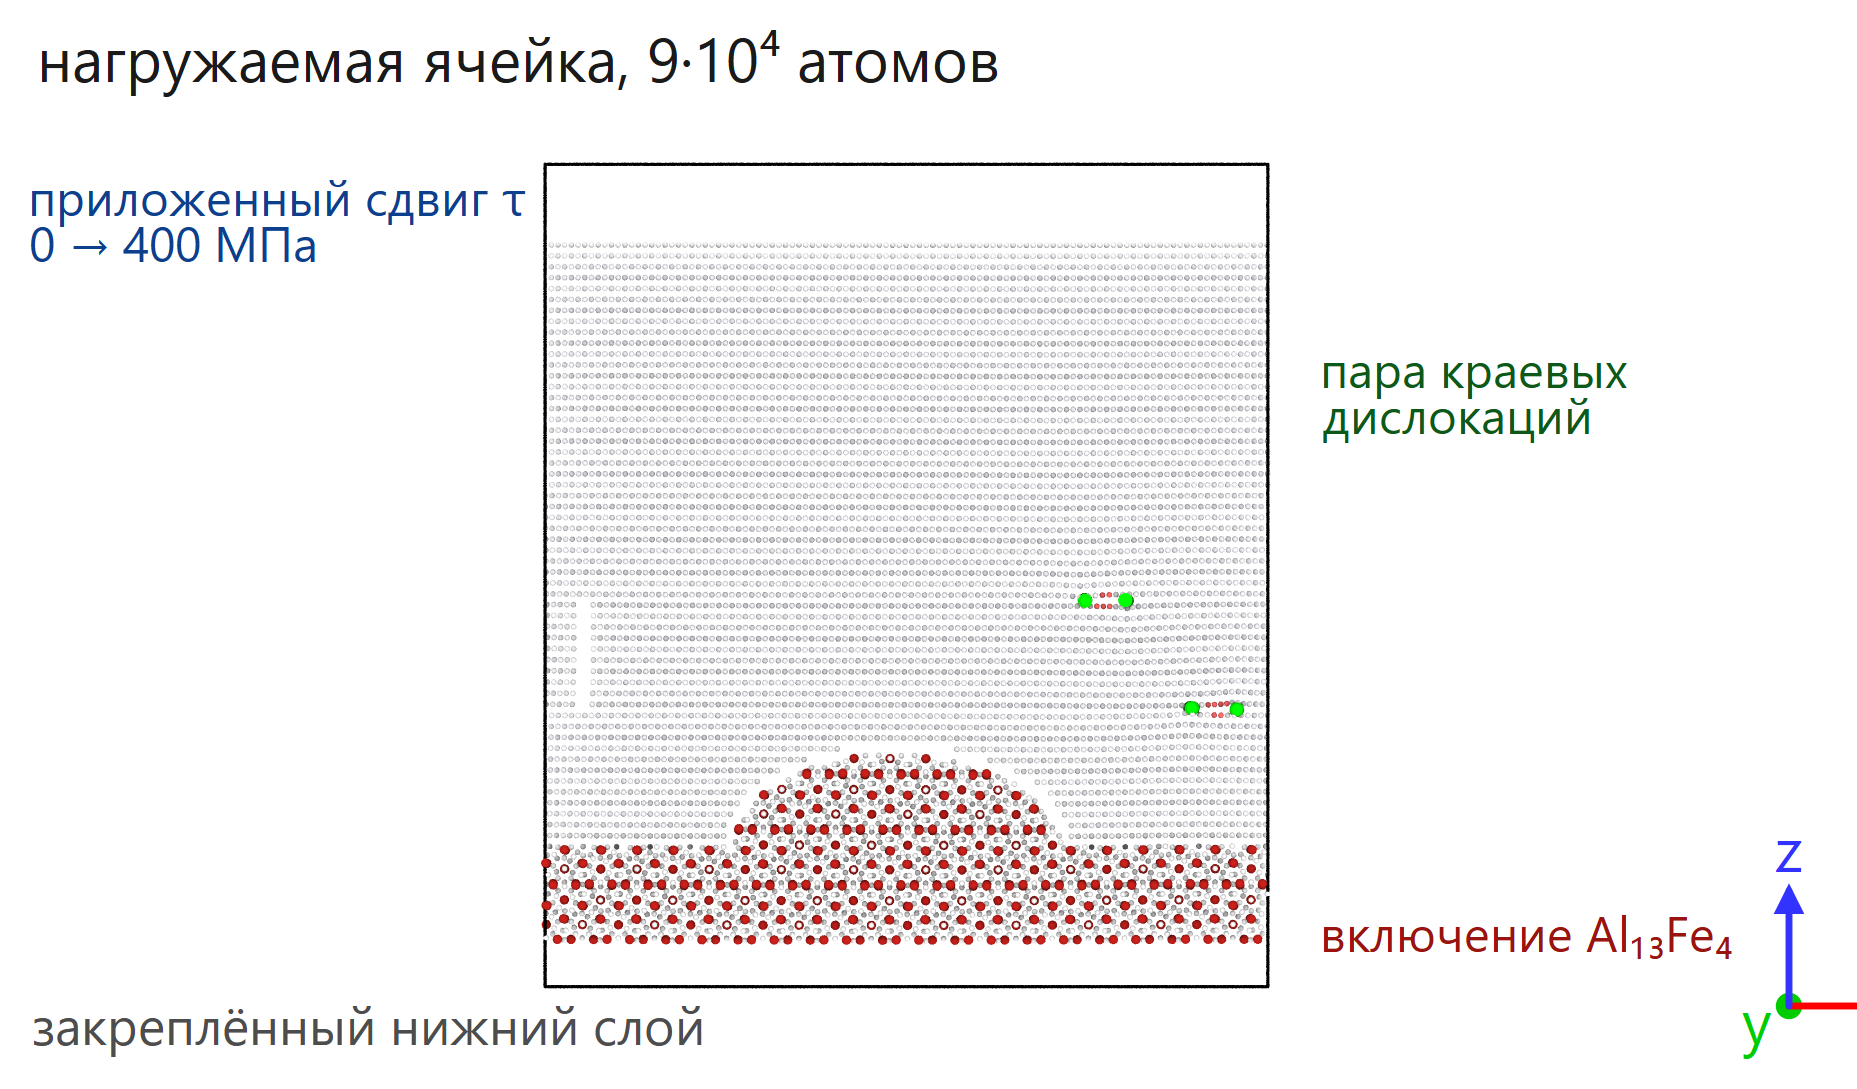
\includegraphics[width=0.92\linewidth]{fig_cell_loading_ru}\\[2mm]
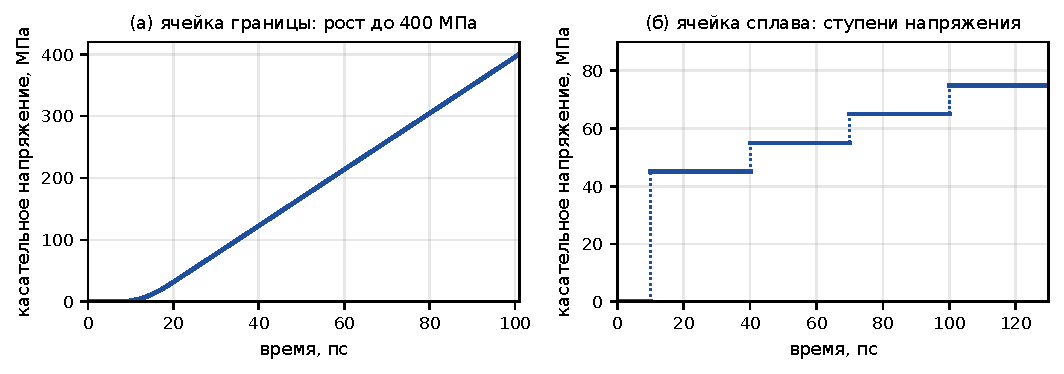
\includegraphics[width=0.92\linewidth]{fig_loading_programme_ru}
\caption{Нагружаемая ячейка границы (вверху) и две программы нагружения
(внизу). Вверху: ячейка рис.~\ref{fig:cell} с парой краевых дислокаций
противоположного знака рядом с гребнем (зелёным показаны линии дислокаций,
найденные дислокационным анализом; атомы совершенной решётки приглушены), обе
в плоскостях скольжения (111), параллельных границе. Касательное напряжение
$\tau$ вдоль $x$ прикладывается однородной силой к верхним атомным слоям и
воспринимается закреплённым нижним слоем. Внизу: программы напряжения --- для
этой ячейки линейный рост от 0 до 400~МПа за 96~пс после 5~пс при нулевом напряжении (удерживаемые ячейки нагружались с той же скоростью до 145~МПа) (а); для ячейки сплава без включения (раздел~3.3) ступени 45, 55,
65 и 75~МПа по 30~пс каждая после 10~пс без нагрузки (б).}
\label{fig:loading}
\end{figure}

\subsection{Вычисление напряжений}

Локальные напряжения получены из поатомного вириального напряжения ---
атомного аналога механического напряжения, вычисляемого для каждого атома из
сил между ним и его соседями и делённого на атомный объём
$\Omega = 16{,}61$~\AA{}$^3$: $\sigma_{ij} = -\langle W_{ij}\rangle/\Omega$.
Напряжение отдельного атома испытывает тепловые флуктуации в несколько ГПа,
поэтому никакая скалярная мера не образуется поатомно. Сначала шесть
компонент тензора усредняются по слою толщиной 4~\AA{}, параллельному границе
(а в динамических расчётах --- и по кадрам), и лишь затем из усреднённого
тензора образуются две скалярные меры: напряжение фон Мизеса --- единственное положительное число,
характеризующее сдвиговую часть напряжённого состояния и входящее в критерий
текучести пластичного металла, --- и разрешённое
касательное напряжение --- касательное напряжение, действующее на данной
плоскости скольжения в данном направлении скольжения. Через
$\mathrm{RSS}_{\max}$ обозначено наибольшее разрешённое касательное
напряжение среди двенадцати систем скольжения $\{111\}\langle110\rangle$
матрицы, то есть касательное напряжение на наиболее благоприятно
ориентированной системе.

Профили напряжений $\sigma(r)$ строятся как функции расстояния $r$ от
плоскости границы по слоям толщиной 4~\AA{} только по атомам матрицы,
лежащим выше вершины гребня, так что $r$ измеряет расстояние от поверхности
включения. Поле деформированного включения есть разность между
деформированной и контрольной ячейками, слой за слоем. В структурах после
минимизации энергии теплового движения нет, и уровень шума этой разности
задаётся остаточным разбросом от слоя к слою вдали от границы: по области
$r \geq 60$~\AA{} среднее $\Delta\mathrm{RSS}_{\max}$ составляет
$2{,}5 \pm 0{,}5$~МПа (среднее и стандартное отклонение по тринадцати
слоям) --- разрешающая способность расчёта, ниже которой поле не
разрешается.